\section{Quadrature Encoder Input}

The quadrature encoder input (QEI) module is provided with a library for both running the thread that handles the direct interface to the pins and also for retrieving and calculating the appropriate information from that thread. 

This module is not explicitly utilised in the current reference design, but could be utilised in the `decoder' thread.

The particular interface that is implemented utilises three signals comprising of two quadrature output (\verb=A= and \verb=B=) and an index output (\verb=I=). \verb=A= and \verb=B= provide incremental information while \verb=I= indicates a return to 0 or origin. The signals \verb=A= and \verb=B= are provided out of phase so that the direction of rotation can be resolved.

\begin{figure}[h]
\begin{center}
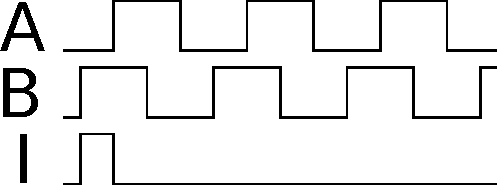
\includegraphics{images/QeiOutput.pdf}
\caption{The quadrature encoder input signals}
\label{fig_QeiInputSignals}
\end{center}
\end{figure}

\subsection{Configuration}

The QEI module requires the following defines in \verb=dsc_config.h=

\begin{lstlisting}
#define QEI_CLIENT_COUNT 2

#define QEI_LINE_COUNT 1024
\end{lstlisting}

The \verb=QEI_CLIENT_COUNT= defines the number of clients that the server supports. This must be a minimum of 1.

The \verb=QEI_LINE_COUNT= defines the number of lines the encoder is specified to have. If this is not defined then 1024 is assumed (as used in the example calculations below). This only affects calculations done by the client functions.

\subsection{QEI Server Usage}
To initiate the service the following include is required as well as the function call shown. This defines the ports that are required to read the interface and the channel that will be utilised by the client thread.

\begin{lstlisting}
#include "qei_server.h"

void do_qei( chanend c_qei[QEI_CLIENT_COUNT],
	port in pQEI);
\end{lstlisting}

\subsection{QEI Client Usage}
To access the information provided by the quadrature encoder the functions listed below can used.

\begin{lstlisting}
#include "qei_client.h"

int get_qei_position( chanend c_qei );

int get_qei_speed( chanend c_qei );

int qei_pos_known( chanend c_qei );

int qei_cw( chanend c_qei );
\end{lstlisting}

Position value is returned in tenths of a degree and speed is returned in revolutions per minute (RPM). 

The third function provides the ability to request whether the QEI interface has received an index signal and is therefore confident that an accurate position can be calculated. Until this function returns 1 then only speed information will be valid.

The fourth function will provide a result of 1 if the direction of rotation of the encoder is clockwise.

\subsection{QEI Service Implementation}
The core functionality is shown below in the state machine in figure \ref{fig_QeiStateMachine}. When in a static state the state machine can be interrupted by a request for rotation data.

\begin{figure}[p]
\begin{center}
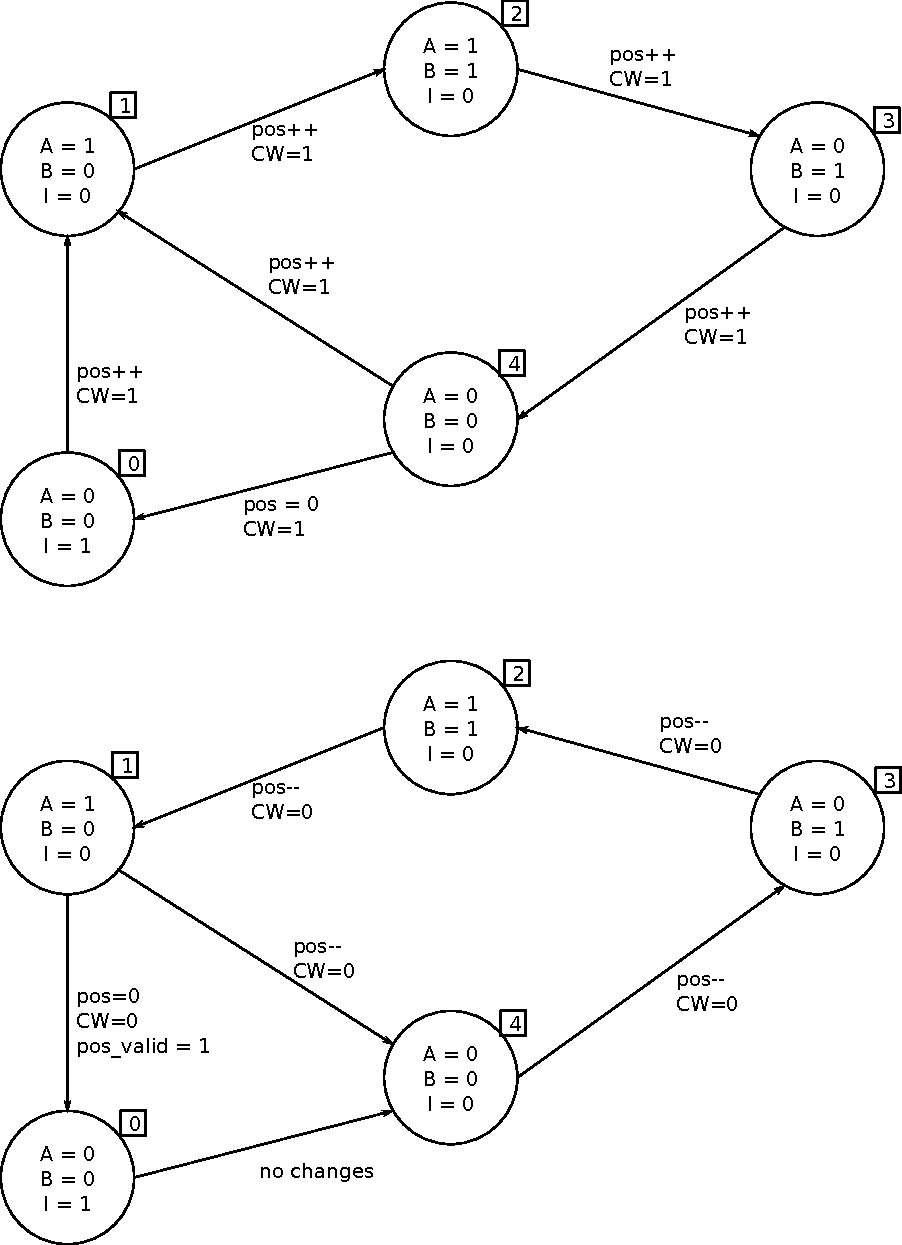
\includegraphics[height=0.9\textheight]{images/qei-state.pdf}
\caption{The QEI state machine showing clockwise and counter clockwise rotation}
\label{fig_QeiStateMachine}
\end{center}
\end{figure}

The request for data will only be served if the event on the channel is enabled. This means that during any state updates the provision of the required data will be a blocked request.

Initialisation of the state machine is done by reading the pins at startup and entering the appropriate state. It is key to note that the position is entirely unknown until an index signal is received, the control algorithm must take account of this. Information as to whether an index value has been received can be queried from the service.

To enable the calculation of both speed and position the time between transitions is recorded and the direction is recorded (as shown for clockwise rotation in the state diagram in figure \ref{fig_QeiStateMachine}).

Communication of the required information is done by the client first requesting the information. This can be requested using the following command values.

\begin{lstlisting}
QEI_CMD_POS_REQ
QEI_CMD_SPEED_REQ
QEI_CMD_POS_KNOWN_REQ
QEI_CMD_CW_REQ
\end{lstlisting}

These are utilised by the client library functions discussed below.

\subsection{QEI Client Implementation}
The client library as described above makes requests to the QEI service thread. These requests are made exclusively via channels and may be blocked during a change in state, but will then be serviced appropriately.

The service thread provides speed and position data in the form of the raw count and time information. This means that to calculate the speed of rotation equation \ref{eqn_QeiSpeed} is utilised on the client side.

\begin{equation}\label{eqn_QeiSpeed}
SPEED =  \frac{60000000}{(t_2 - t_1) \times 1024}
\end{equation}

Calculation of position in tenths of a degree is also performed on the client side and is shown in equation \ref{eqn_QeiPosition}

\begin{equation}\label{eqn_QeiPosition}
POS = (QEI\_RAW\_POS \times 3600) >> 10 
\end{equation}

Direction and whether an index signal has been received are direct values presented as requested from the QEI service.
